\renewcommand{\thechapter}{\roman{chapter}}
\setcounter{chapter}{3}
\setcounter{figure}{0}

\unchapter{Préambule microscopie confocale par réflectance}
\label{chap:preamble_microscopy}
Au sein de cette seconde partie, nous élaborerons une méthodologie destinée à la modalité \gls{rcm}. Les éléments nous ayant conduits à nous intéresser à cette modalité sont multiples. En premier lieu, il s'agit de l'une des modalités les plus précises en notre possession, elle consiste donc en une référence en terme de qualité de diagnostic à réaliser. Enfin, le nombre restreint de travaux menés sur le diagnostic de lésion de la peau appliqué au \gls{rcm} assisté par ordinateur est un second argument. En effet, cette modalité représente pour nous un verrou scientifique que nous devons lever pour accomplir le schéma de diagnostic multimodal. Ce préambule à destination de la modalité \gls{rcm} a pour objectif de présenter les données de travail exclusives à cette modalité et à présenter les objectifs que nous nous fixons par l'apport des méthodes d'aide au diagnostic que nous réaliserons.\par

Ainsi, dans cette partie ne seront considérées que les données \gls{rcm} des 223 lésions en notre possession et sont donc exclues les images de photographie clinique et de dermatoscopie. Également, ont été utilisés 28 patients bénins non présents dans la base d'images initiale afin d'augmenter le nombre d'images annotées comme bénignes. Ces images comportent également des lésions pouvant porter a confusion lors du diagnostic de \gls{lm}/\gls{lmm} par le spécialiste. Ces données seront utilisées uniquement dans le but de renforcer l'entraînement.\par

Les données \gls{rcm} de chaque lésion contiennent essentiellement des images jugées pertinentes par deux des trois médecins investigateurs et provenant de l'épiderme, de la \gls{dej} et du derme. Néanmoins, les données utilisées ici correspondront essentiellement à des données de la \gls{dej}. En effet, le \gls{lm}/\gls{lmm} sont des pathologies de la peau caractérisées par l'intrusion de la mélanine se propageant le long des follicules pileux. Les images de la \gls{dej} sont ainsi parfaitement adaptées à l'observation de ce phénomène par les médecins.\par

Du point de vue de leurs caractéristiques, ces images arborent une taille constante de \SI{1000}{\px} $\times$ \SI{1000}{\px} pour une section mesurée de \SI{920}{\micro\metre} $\times$ \SI{920}{\micro\metre} pour une résolution en profondeur comprise entre \SIrange{3}{5}{\micro\metre}. Ces données fournissent ainsi une résolution de l'ordre du \SI{1}{\micro\metre}. Les informations d'acquisition (profondeur, longueur d'onde, \ldots) contenues dans les images ne pourront être utilisées car non exploitables (procédure de calibration non réalisée, informations manquantes, \ldots).\par

A partir de ces données, les 18 experts en \gls{rcm} de l'étude~\cite{Cinotti2018} ont obtenu en moyenne une sensibilité de 0,84$\pm$0,05 et une spécificité de 0,75$\pm$0,06 sur l'évaluation des pathologies malignes toutes confondues. Sur l'évaluation des données de \gls{lm} et \gls{lmm}, ces scores sont de 0,80$\pm$0,07 et 0.81$\pm$0,05. Les courbes \gls{roc} associées à ces performances sont représentées sur la \Cref{fig:results_rcm_experts}.\par

\begin{figure}[H]
    \begin{center}
        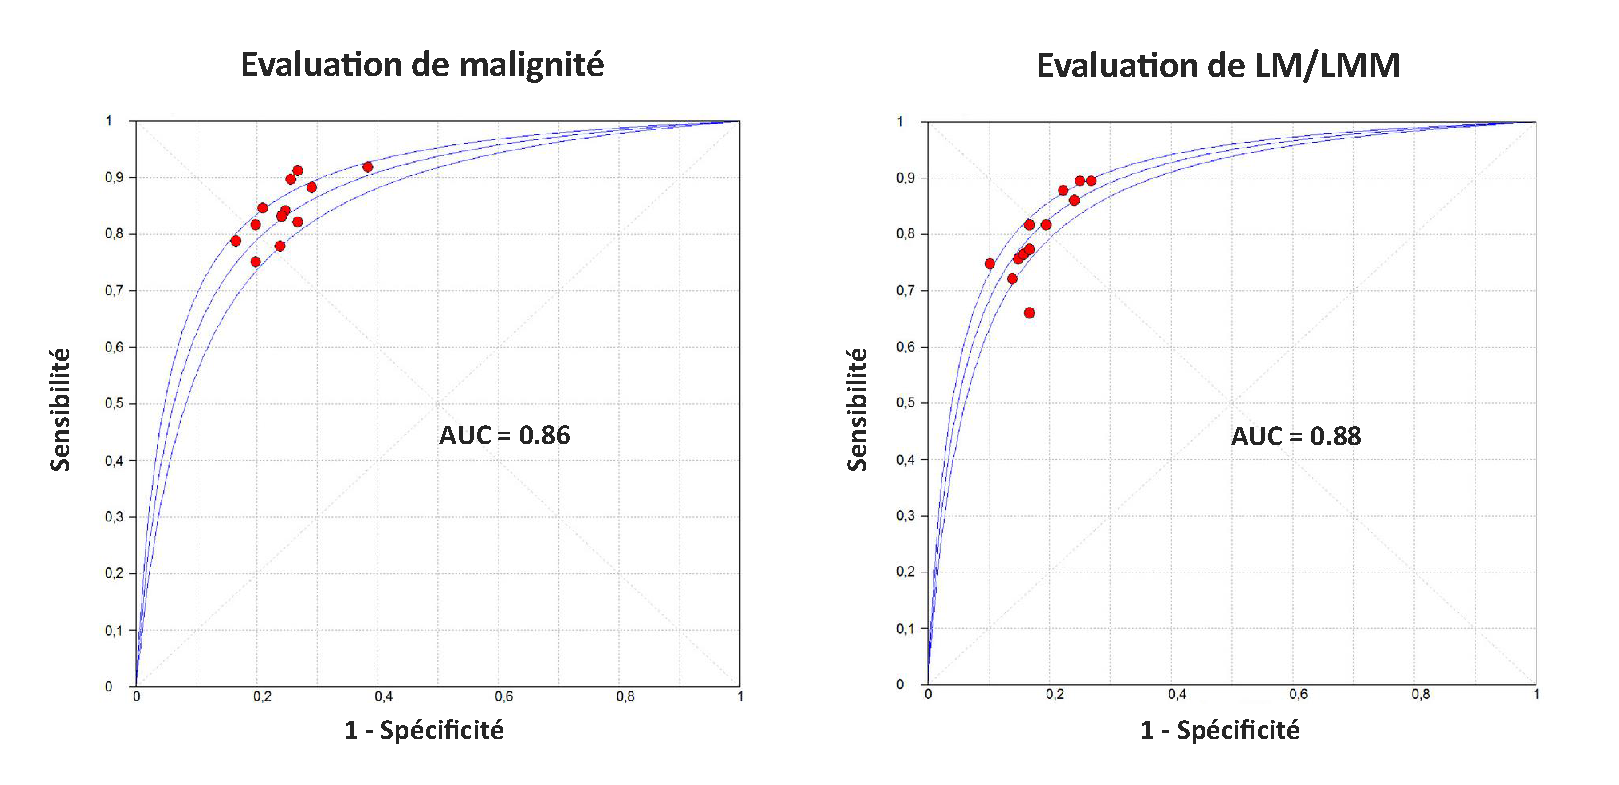
\includegraphics[width=\linewidth]{contents/ii_preamble_microscopy/resources/results_rcm_experts.pdf}
        \caption{Courbes \gls{roc} issues de l'évaluation des données \gls{rcm} par les 18 experts~\cite{Cinotti2018}. A gauche, le résultat des experts mené sur la détection d'éléments malins ; A droite, le résultat des experts mené sur la détection de \gls{lm} et \gls{lmm}.}
        \label{fig:results_rcm_experts}
    \end{center} 
\end{figure}\par

L'objectif visé par cette partie sera d'égaler ces scores à l'aide de nos méthodes de diagnostic sur base d'images issues de \gls{rcm}. A ce titre, nous n'exploiterons pas les méta-données issues des informations patient bien que utilisées par les spécialistes lors de l'évaluation. Ainsi, l'âge, le sexe ou encore l'emplacement sont autant de critères que nous ne considérerons pas au sein de ces prochains paragraphes bien que employés par les dermatologues experts en \gls{rcm} durant leur évaluation. De plus, contrairement aux connaissances des experts, ces méta-données ne sont pas représentatives de la population réelle, et biaiseraient nos méthodes par des corrélations non valides dans le monde réel dû à l'acquisition de la base de données.\par

\begin{figure}[H]
\centering
    \begin{subfigure}{.45\textwidth}
      \centering
      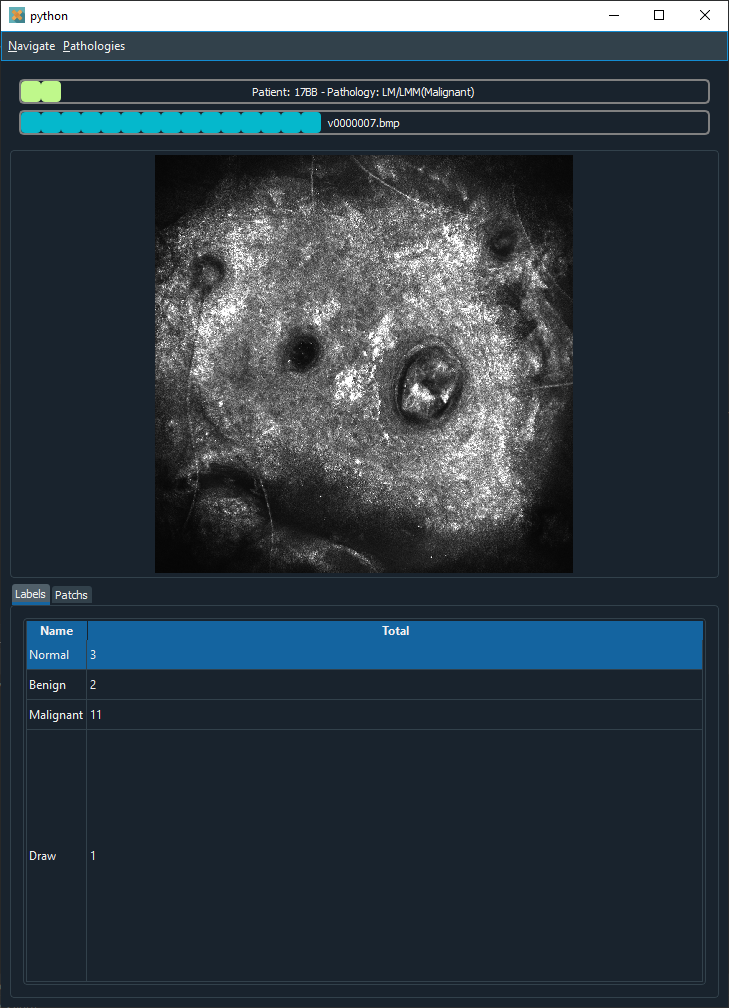
\includegraphics[width=0.8\linewidth]{contents/ii_preamble_microscopy/resources/example_gui_annotation_1.png}
    \end{subfigure}
    \begin{subfigure}{.45\textwidth}
      \centering
      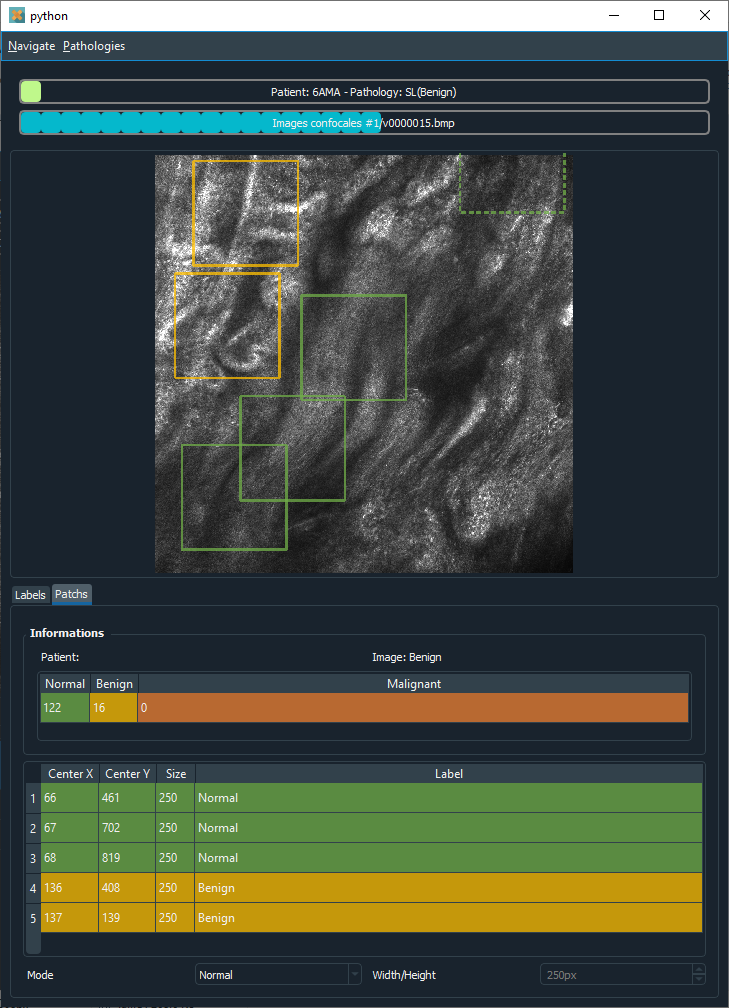
\includegraphics[width=0.8\linewidth]{contents/ii_preamble_microscopy/resources/example_gui_annotation_2.png}
    \end{subfigure}
    \caption{Interface logicielle mise à disposition du spécialiste, afin de procéder aux annotations. A gauche, l'onglet permettant l'annotation au niveau des images, à droite l'onglet permettant la création de patchs.}
    \label{fig:example_gui_annotation}
\end{figure}

Ainsi, nous sollicitons diverses ressources d'intelligence artificielle évoquées lors du \Cref{chap:chapter_3}. Des apports ont été réalisés pour permettre le déroulement des expériences que nous présenterons lors des chapitres suivants. En effet, la base d'images actuelle ne possède que des annotations au niveau des patients, ce qui limite fortement nos travaux essentiellement basés sur de l'apprentissage supervisé. A l'aide d'un outil graphique réalisé pour cette étude (\Cref{fig:example_gui_annotation}), nous avons pu obtenir grâce au travail de l'un des dermatologistes investigateur :
\begin{itemize}
    \item des annotations au niveau des images,
    \item des annotations au niveau de sous parties d'images ou \textbf{patchs}.
\end{itemize}\par

Des annotations selon 3 critères se sont naturellement imposées pour ces deux tâches. Une annotation de type \textit{malin} a été apposée sur des images contenant \textbf{au moins} du tissu de type malin et, sur des sous-images composées de ce type de tissus. Selon ce même schéma, une annotation de type \textit{bénin} a été apposé sur des images ne contenant \textbf{aucun} tissus malin mais \textbf{au moins} du tissu bénin et, sur des sous-images composées de ce type de tissus. Enfin, une annotation de type \textit{sain} a été renseignée sur des images ne contenant \textbf{aucun} des deux types de tissus précédents et sur des sous-images composée de tissus sains. Des exemples d'images et annotations selon ces 3 critères sont disponibles sur la \Cref{fig:example_rcm_data}.\par

\begin{figure}[H]
    \begin{center}
        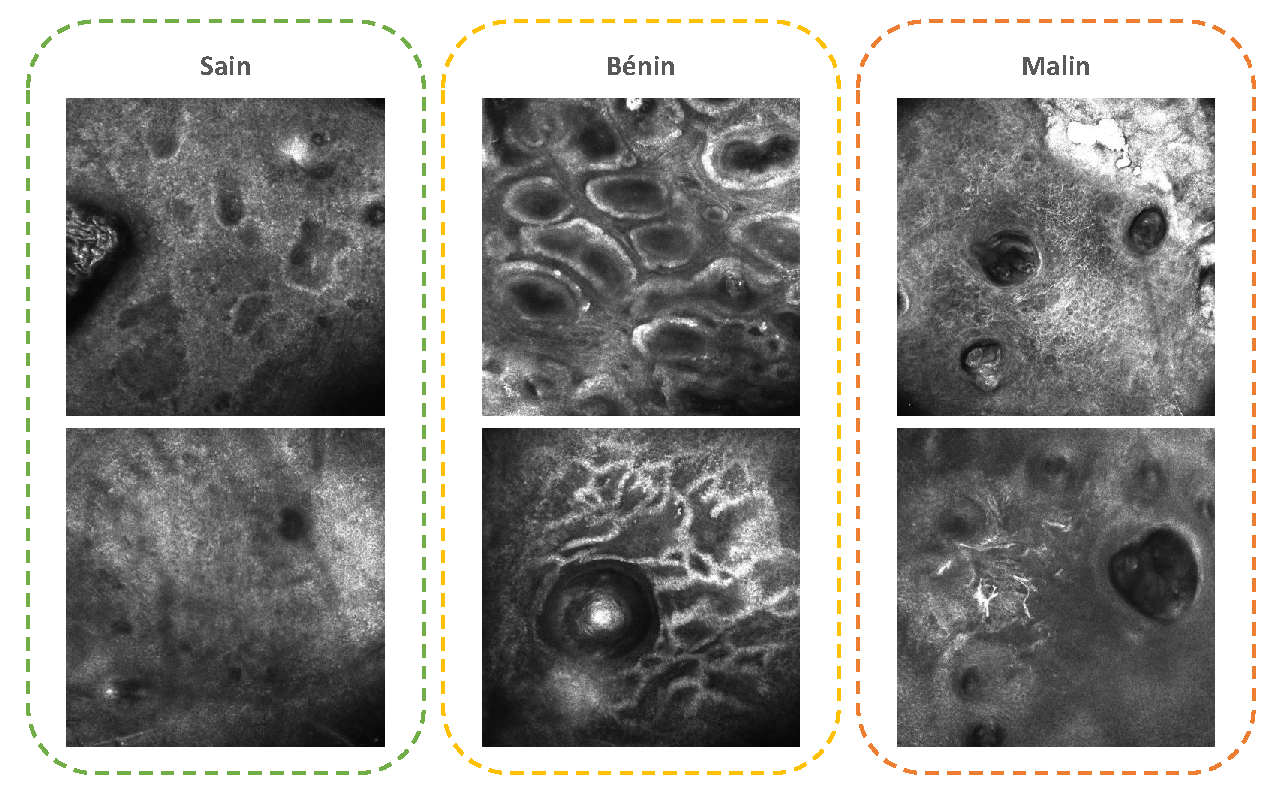
\includegraphics[width=\linewidth]{contents/ii_preamble_microscopy/resources/example_rcm_data.pdf}
        \caption{Exemple de tissus et annotations, considérés respectivement de gauche à droite comme \textit{sain}, \textit{bénin} et \textit{malin} par le spécialiste.}
        \label{fig:example_rcm_data}
    \end{center} 
\end{figure}\par

La répartition complète de cette base annotée peut être visualisée sur la \Cref{fig:scheme_rcm_statistics}. Nous pouvons y visualiser la composition de la base d'image et celle des sous-images ou patchs. La couleur bleu permet de visualiser le jeu de données initial servant à l'entraînement et l'évaluation~\cite{Cinotti2018}, et en orange les données servant à corriger partiellement le non balancement.\par

\begin{figure}[H]
    \begin{center}
        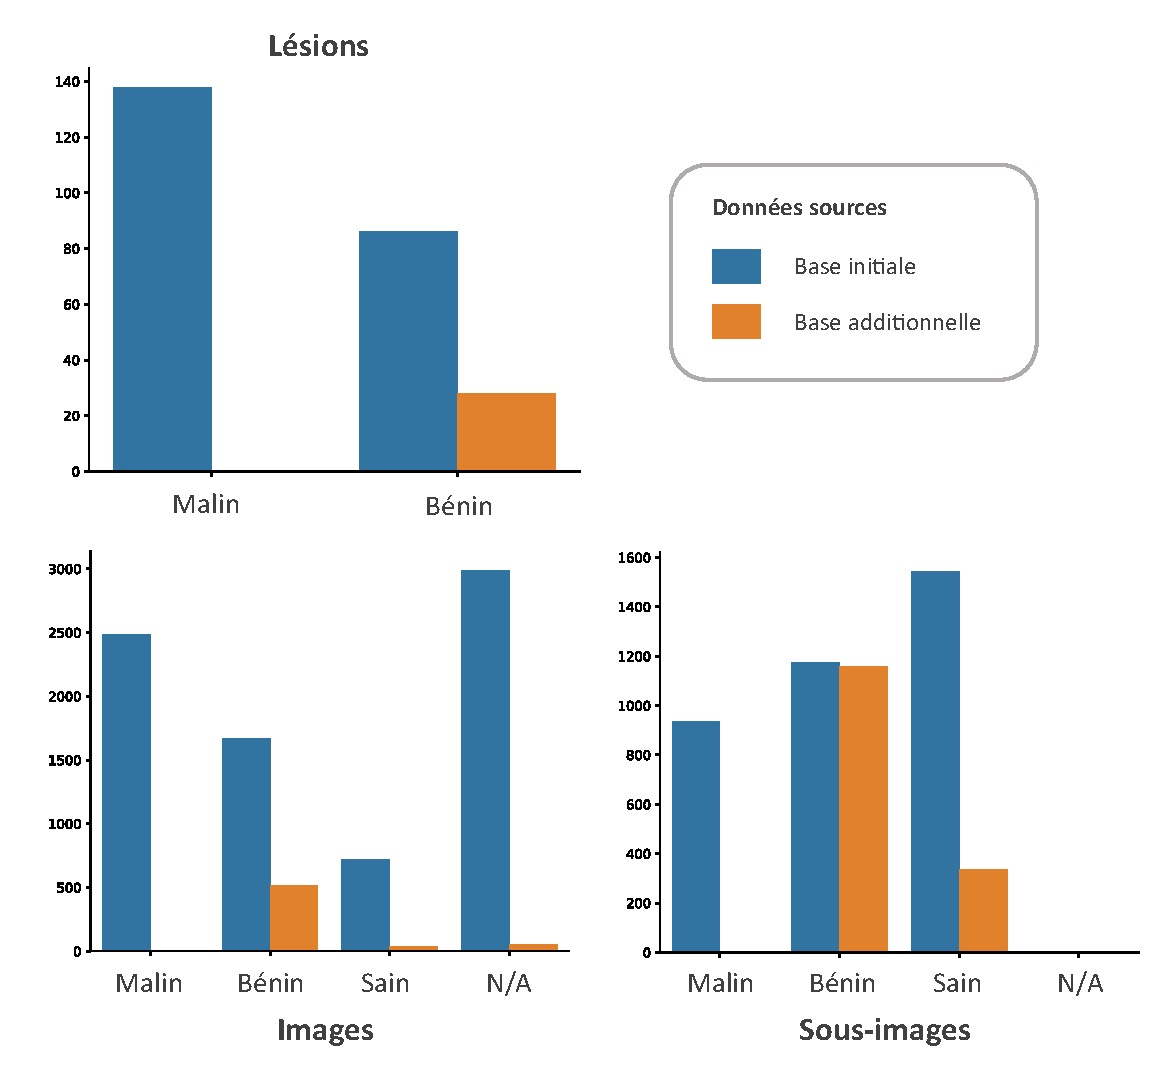
\includegraphics[width=\linewidth]{contents/ii_preamble_microscopy/resources/scheme_rcm_statistics.pdf}
        \caption{Répartition des annotations réalisées par l'expert, en bleu sur la base initiale de Cinotti~\cite{Cinotti2018} et en orange sur les données bénignes supplémentaires. A gauche, la répartition des annotations images ; A droite, la répartition des annotations sur les sous-images.}
        \label{fig:scheme_rcm_statistics}
    \end{center} 
\end{figure}\par

Afin de répondre à ce besoin, cette partie dédiée au \gls{rcm} se compose de trois chapitres dans lesquels nous élaborerons une méthodologie ascendante :
\begin{inlinerate}
    \item le premier chapitre abordera la \textbf{prise de décision au niveau de l'image},
    \item le second chapitre proposera des méthodes destinées à \textbf{améliorer ce diagnostic image},
    \item enfin le dernier chapitre de cette section se focalisera sur une \textbf{prise de diagnostic au niveau du patient}.
\end{inlinerate}\par
\newpage